% Styling commands for the used terms
\newcommand{\agent}{{\tt agent}}
\newcommand{\entity}{{\tt entity}}
\newcommand{\activity}{{\tt activity}}
\newcommand{\relation}{{\tt relation}}
\newcommand{\relations}{{\tt relations}}
\newcommand{\attributes}{{\tt attributes}}

\section{Data Provenance}
\label{datamodel-provenance}

A topic with growing interest in the \escience{} field is provenance, sometimes also referred to as lineage or pedigree.
It has been borrowed from the world of art where it describes the `life' of an artwork.
Mostly this will be the record of ownership but it can also describe things like restorations.
From provenance data the quality, state, and originality of the work can be discerned.

In \escience{} the same can be applied on a piece of data \cite{dsp4moreau}.
Concerning data, provenance is stored metadata describing the process by which the data got to a certain state from a specific source \cite{dsp4moreau,dsp2buneman}.
To describe the path data has taken W3C has made a standard described in the PROV Model Primer \cite{dsp8gil}.
The gist of provenance is that it is build from a small set of assertions made by the different services that are involved in  the data process \cite{dsp4moreau}.
To actually \emph{use} provenance data a standard for schemas is described which are usable for human consumption, an example is shown in figure \ref{fig:provenance-large-schema}.

Provenance is explored here because it can be considered as an extension on data security.
Since provenance directly monitors data and is consumable by humans it provides another level of security compared to the previously described solutions in \ref{security-summarisation}.

%TODO extra information about schemas, surplus/confusing
%Because these schemas can run from the starting point where provenance data was kept (or actually the beginning of all time) user-tailored queries should be applied \cite{dsp4moreau}.
%These frame the specific question a user has and only display the applicable part of the schema.

\paragraph{The `why?' of provenance}
\label{provenance-why}

When collecting provenance various metadata has to be captured at different steps in the data process.
This creates a overhead when using a system for a specific task.
Capturing and keeping provenance data is almost never the main functionality of a system.
However, exposing the data may help users (\ie{} researchers).

In \escience{} data is gathered and generated at a fast pace.
Provenance kept of this data can help researchers determine whether data is:

\begin{itemize}
	\item Usable in a certain context, the metadata stored can describe the different uses of a specific data item \cite{dsp1simmhan}, \eg{} types of software that accept a data item as input.
	\item Acceptable, a researcher can discern from provenance whether to trust the accuracy and timeliness and accept if for further use \cite{dsp1simmhan,dsp3buneman}.
	\item Protected by intellectual property (IP) or should be credited, as for the acceptability of data the path can also be backtracked to the original creators and/or IP holders \cite{dsp1simmhan}.
\end{itemize}

\paragraph{The `how?' of provenance}
\label{provenance-how}

The provenance building blocks (as described by the W3C \cite{dsp8gil}) consist of three core data types (\agent{}, \entity{}, and \activity{}) and \relations{} between them.
Furthermore, \attributes{} can be assigned to provide metadata for data types or \relations{}.
Figure \ref{fig:provenance-overview} shows the standardised display methods for the data types and \relations{}, \attributes{} are displayed with a `document' symbol as shown in figure \ref{fig:provenance-large-schema}.
Also, an applied provenance example is given in figure \ref{fig:provenance-large-schema}.

\begin{figure}[!tbhp]
	\centering
	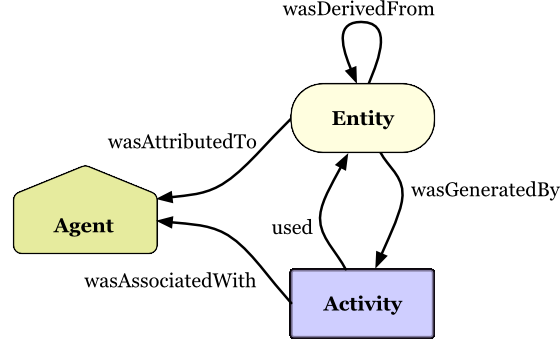
\includegraphics[width=0.5\linewidth]{images/provenance-overview}
	\caption{Example model showing the three core data types (\agent{}, \entity{}, and \activity{}) and a few of all possible \relations{} between them. 
		Taken from PROV Model Primer \cite{dsp8gil}.}
	\label{fig:provenance-overview}
\end{figure}

List of used concepts as described in PROV Model Primer \cite{dsp8gil}:

\begin{itemize}
	\item Entity, physical, digital, conceptual, or another type of `thing'.
	\item Activity, the process of instantiating or the process of changing an entity.
	\item Agent, holds (a part of) the responsibility for activities and entities.
	\item Relation, describes the interaction between two instances of the data types.
\end{itemize}

\begin{figure}[!b]
	\centering
	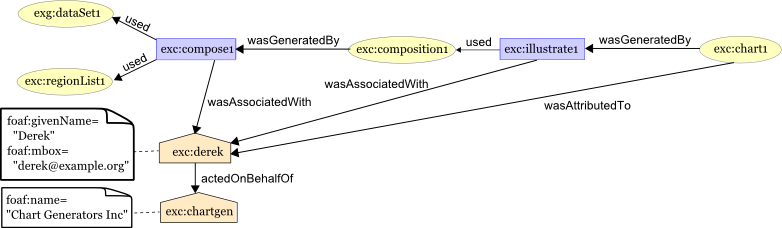
\includegraphics[width=1.0\linewidth]{images/provenance-large-schema}
	\caption{
		Real life example model which implements the model as shown in figure \ref{fig:provenance-overview}.
		This example describes the creation of a chart, the original data used, the intermediate data generated during the process, the used software, who was responsible for the work, and who this person was working for.
		An addition to figure \ref{fig:provenance-overview} is the use of \attributes{}, these are displayed with document icons and provide metadata on the object they are related to.
		In this case that is the name and email address for one the agents and the company name for the other agent.
		Taken from PROV Model Primer \cite{dsp8gil}.
		}
	\label{fig:provenance-large-schema}
\end{figure}

%TODO explanation of figure, unnecessary as it is already in caption and explains itself?
%An applied provenance example is given in figure \ref{fig:provenance-large-schema}.
%This figure shows what the provenance of a certain `chart' is.
%The chart (\entity) is shown at the far right side of the figure; it was generated by (\relation) some illustration software (\activity); which in its turn used data from a composition dataset; the data was generated by composing software; two datasets were used in the process, data set 1 and region list.
%The agent executing this process is Derek (\agent), he was associated with the composing and illustration software and is attributed to the creation of the resulting chart.
%However, Derek is acting on behalf of the company chart gen (\eg{} he is a contractor or employee).
%Both agents in this example have \attributes{} assigned to them to further describe them (\eg{} the full name of the company).

\paragraph{The use of provenance in security}
\label{provenance-use}

Three types of assertions can be described which account to provenance: relationship (object B was retrieved by applying function X to object A), interaction (received object A, sent object B), and service state (it took three seconds to send object B after receiving object A) \cite{dsp4moreau}.

Different applications of provenance can be accomplished with these assertions \eg{} data quality, audit trail, replication recipes, attribution, and informational \cite{dsp1simmhan}.
Data quality uses the provenance metadata as a check, like described with the art example at the beginning of this subsection, the user tries to discover who did what with the data.
The same applies for an audit trail, but it is used for other ends, being able to maintain responsibilities.
Replication recipes are an extension of data quality, a user can execute the exact same steps on the same or a different piece of data to check the work or to improve on the work done.
In the case of data ownership attribution can be used to trace who should be contacted for consent on data usage.
Lastly, informational provenance helps with data discovery and providing context for data, which helps with (for example) reuse.

There are many applications of provenance in security, different levels can be supplied by mixing computerised surveillance with human insight.
One of the clearest examples is the data audit functionality.
The necessary metadata for an audit is collected automatically during the operation of the system.
Outcomes of this audit can be partly analysed by a computer but can also be translated into an human understandable format.
Further actions that lead to actual security should be captured in standardised processes, therefore provenance is only a tool and not an security end-point.

%TODO implementation details, not necessary here might come back in implementation chapter
%Furthermore, there were three points of interest found regarding the implementation of provenance: data object identifiers, manual versus automated data entry, effect on performance.
%Data object identifiers (DOI) can be used to identify and cite data \cite{dsp1simmhan}.
%When these DOIs are used in publications the provenance can be easily gathered later when an interested party wants to check the process of an experiment.
%If provenance metadata is entered manually be users there is a high risk of losing value from missing values and non-standardised input \cite{dsp1simmhan}.
%Manual versus automated is an issue because of performance, provenance creates a overhead both in computational resources as data storage.
%Therefore, metadata should be gathered and stored on a `piecemeal basis' \cite{dsp4moreau}.